\subsection{Feature of the hierarchical structure}
The control system for a collaborative mini manipulator robot includes other systems, such as motor control, internal and external peripherals, and others, which are interdependent. Therefore, to develop the structural diagram of the control system for a collaborative mini manipulator robot, a hierarchical paradigm of control system architecture for robots was used. According to this paradigm, the hierarchical architecture of the robot control system (Fig. \ref{Hierar}), in general, contains four levels of control: intelligent level, strategic level, tactical level, and executive level \citep{Khatib1997}.

\begin{figure}[H]
	\centering
	\includesvg{Src/images/Hierarchy(1).svg}
	\caption{Hierarchical architecture of the robot control system}
	\label{Hierar}
\end{figure}

In the hierarchical architecture of the manipulator robot control system, the levels of control ensure the performance of specific robot control tasks:

\begin{itemize}
	\item At the intelligent level, decisions are made (formulated) about the actions performed by the manipulator robot under conditions of incomplete information about the external environment and the objects the robot interacts with (for example, moving an object from one point in space to another, processing a part, etc.).
	\item The strategic control level is intended for planning the movements of the manipulator robot: dividing the action task, developed at the intelligent level, into a sequence of temporally coordinated elementary actions (movements) and formalizing the control objectives for each of these actions. The strategic level issues to the tactical level a motion plan in the form of motion control commands. For example, moving the robot's end-effector (gripping device) to a specified position, grasping an object, test movement to determine the reaction forces from the object, moving the object, and returning the robot to its original position.
	\item At the tactical level, the motion control commands coming from the strategic control level are transformed into a control program that defines the laws of coordinated motion over time of all the robot's links, considering the technical characteristics of the drive unit (primarily limitations on generalized velocities, accelerations, and forces). To execute the position control command for the manipulator robot at the tactical level, it is necessary to determine the generalized coordinates of the manipulator that correspond to the desired Cartesian coordinates of the characteristic point of the manipulator robot's gripping device. For this purpose, the inverse kinematic problem of the manipulator's position at a given point of the motion trajectory is solved.
	\item The executive control level is designed to calculate and issue control signals to the manipulator robot's drive unit in accordance with the control program created at the tactical level, considering the technical characteristics of the actuating devices.
\end{itemize}

\subsection{Structure diagram of the mini robot control system}

Figure \ref{Structural} illustrates the structural diagram of the mini robot control system. The control system for the mini manipulator robot has a hierarchical structure that corresponds to the hierarchical architecture of the robot control system (Fig. 2.1), as the developed structural diagram includes devices corresponding to the functions of control levels in (Fig.2.1):
\begin{enumerate}
	\item Strategic Control Device (SCD)
	\item Tactical Control Device (TCD)
	\item Actuator Control Devices (ACD)
\end{enumerate}

The Tactical Control Device (TCD) of the mini robot coordinates the operation of all devices in the mini robot control system, ensuring the efficient functioning of the entire robot mechanism. It processes control commands from the Strategic Control Device (SCD) and is responsible for forming output signals to Actuator Control Devices (ACD), ensuring the robot's behavior corresponds to the given commands.



The Actuator Control Device (ACD) is a device whose main purpose is to generate signals for precise control of a single mechanical device (electric motor), providing rotation of the manipulator robot arm. This device allows for motor control without using the Tactical Control Device (TCD). This enables complex manipulations with a high degree of precision and turning the motor axis to the required angle.
\begin{figure}[H]
	\centering
	\includesvg[width=\textwidth]{Src/images/Main control system(2).svg}
	\caption{Structural diagram of the mini robot control system}
	\label{Structural}
\end{figure}
After receiving data from the Strategic Control Device (SCD), the Tactical Control Device (TCD) sends data to the motor control system of each axis (ACD).

After receiving a motion command, positions and accelerations are calculated, and data is sent to the motion control system (ACD) of each axis. If the controlled parameters go beyond the range of allowed values, an emergency mode is triggered, and information is displayed on the information panel.

The indication panel provides information about current parameters and system states, as well as the robot system's state. The device facilitates monitoring the state of the manipulator robot and ensures quick problem detection by notifying the operator. When the system determines further motion of the robot is impossible, red indicates this, yellow for waiting, and green for operation.

The power supply is an integral element of the system. It converts network electricity, by forming the required current and voltage values (24V), to power all the electrical devices of the robot.

The voltage converter is necessary to change the power supply voltage levels to the required parameters, as different devices have various permissible power supply voltage and current values.

Brushless DC electric motors convert electrical energy into mechanical energy. They provide motion to various axes of the manipulator robot.

The emergency stop device is used for the immediate stopping of the robot in emergency situations, preventing accidents and damage to structures.

The data bus ensures communication between the Tactical Control Device (TCD) and Actuator Control Devices (ACD). This communication allows efficient coordination of all motion control devices (ACD) actions among themselves, as well as simultaneous synchronization during movement.

\subsection{Structural Diagram of the Actuator Control System}

The structural diagram of the axis motion control systems is depicted in Figure \ref{ACD}. The purpose of this system is the direct control of the synchronous motor and monitoring its parameters. The main control elements of the system are the Actuator Control Devices (ACD). Since controlling an electric motor requires signals with frequency and phase regulation, it is the ACD that generates the controlling PWM signals.

Drivers amplify the power of the control PWM signals, thus ensuring the compatibility of the ACD signal with the output power transistors. The drivers allow for timely and safe switching of the inverter transistors.

\begin{figure}[H]
	\centering
	\includesvg[width=\textwidth]{Src/images/Actuator system(1).svg}
	\caption{Structural diagram of the actuator control device}
	\label{ACD}
\end{figure}

The signals supplied to the electric motor are controlled by power switching transistors. The electric motor needs to be regulated by changing the frequency and phase of the signal.

Power transistors form a three-phase bridge voltage inverter, and the operating mode of the transistors is switching. In this mode, the transistors switch between fully open and fully closed states, which ensures high efficiency and minimizes transistor heating, which is especially important when creating a small-sized device.

The formation of PWM signals is carried out using the values of the current rotation angle of the axis, acceleration, and torque on the motor. By changing the width of the PWM pulses, the ACD control system can regulate the amount of energy supplied to the motor, thereby changing the speed and torque parameters.

The voltage converter provides the formation of supply voltages for various devices. The type of converter is a DC/DC converter, and the converted voltage is the 24V voltage from the common power source. The system contains various components with different levels of supply voltage, so supplying the power voltage from the outside is not an efficient method.

The data bus allows for data transmission between different devices by connecting components into a single network. Thanks to the use of the network, it becomes possible to exchange data with one or several devices simultaneously.
\subsection{Algorithm of the Tactical Control Device Operation}

Figure \ref{AlgTCD} shows the main algorithm for the Tactical Control Device operation, whose main task is to control the motor of a single robot axis. By default, when the system is turned on, the system initialization takes place, which involves checking the communication functionality between devices and verifying the non-critical state of each ACD and motor. As the final step, the indication panel parameters are initialized and set.


\begin{figure}[H]
	\centering
	\includesvg[width=\textwidth]{Src/images/Main Controller algorithm.svg}
	\caption{Algorithm of the Tactical Control Device operation}
	\label{AlgTCD}
\end{figure}


If the connection with the motors and the ACD interface has not been normalized, the control system will remain in standby mode until the connection is restored. After successfully connecting to all robot devices, commands are set and sent to the ACD actuator devices, setting the minimum values of speed, angle, and acceleration of rotation for each robot axis. Since the position of the robot's axes after the previous shutdown is unknown, it is necessary to calibrate all axes. Calibration occurs after receiving a permission command from the Strategic Control Device (SCD).

In the system's operation mode with the robot's powered-on flag raised, after receiving the respective command, the angles of each axis are read, and commands are sent to the ACD depending on the calculations made. Thus, the Strategic Control Device (SCD) does not participate in the path-building calculations but only sends data to the Tactical Control Device (TCD).

The "Parse command" algorithm is illustrated in Figure \ref{AlgParse}. After receiving a command from the (SCD), the movement type calculation is executed.

\begin{figure}[H]
	\centering
	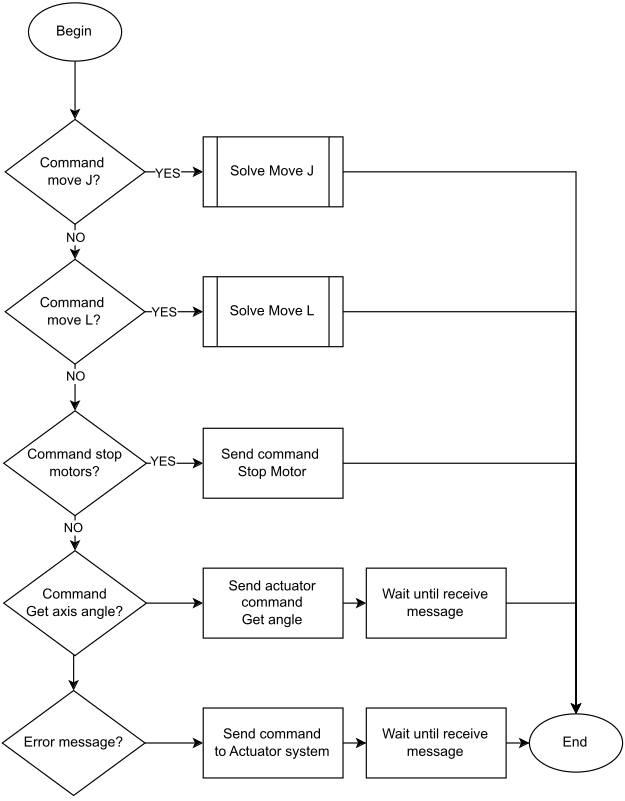
\includegraphics[width=0.7\textwidth]{Src/images/parse.png}
	\caption{"Parse command" algorithm}
	\label{AlgParse}
\end{figure}
The calculation includes a set of algorithms for linear (Move L) and axial (Move J) movements. In case of receiving commands related to the robot's actions, such as data on rotation angles or torque of each axis, the system sends a command to poll the ACD devices. The TCD device waits for confirmation of the sent command (ACK command). After that, the "Parse command" algorithm application ends, and the transition to "Make calculation" occurs.

The main subroutine for calculating the motion trajectory is the "Move J" command illustrated in Figure \ref{AlgJ}. The essence is to perform the movement to a specific position in the fastest way using angular movements. In the implementation of this function, accelerations for each robot axis are calculated, but only if the angles of the planned point are within permissible values.

\begin{figure}[H]
	\centering
	\includesvg[width=0.8\textwidth]{Src/images/Move J.drawio(1).svg}
	\caption{"Move J" subroutine algorithm}
	\label{AlgJ}
\end{figure}

The subroutine for calculating the motion trajectory is the "Move L" command (Figure \ref{AlgL}), for the robot's arm. The set of algorithms solves the inverse problem, the result of which is several position options, rotation angles of the robot's links. Next, a list of robot position options that do not exceed the physical limits of each robot axis is formed. Also, the calculation of the smallest angle from the initial position of the robot is required.

\begin{figure}[H]
	\centering
	\includesvg[width=0.8\textwidth]{Src/images/Move L.drawio.svg}
	\caption{"Move L" subroutine algorithm}
	\label{AlgL}
\end{figure}

\subsection{Algorithm of the Actuator Control Device Operation}

The algorithm for the Actuator Control Device is demonstrated in Figure \ref{AlgACD}. 


\begin{figure}[H]
	\centering
	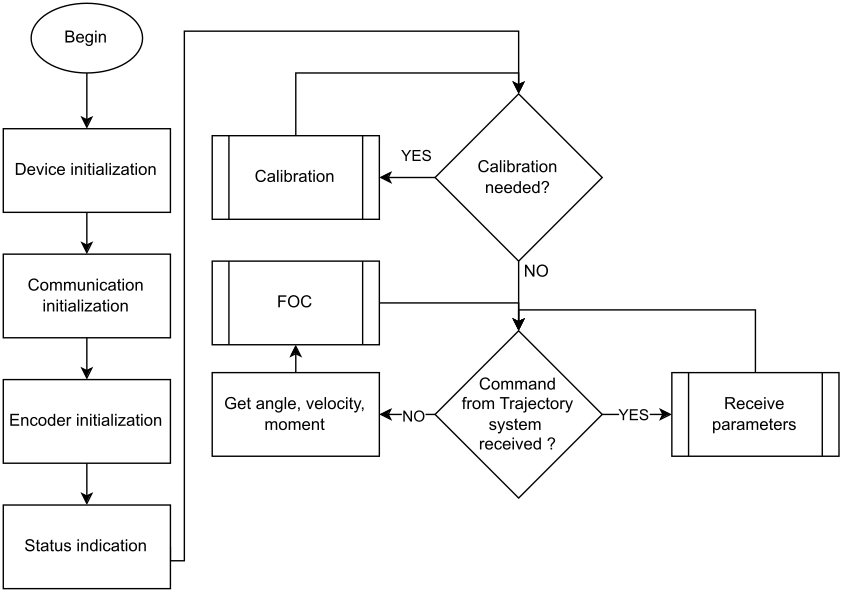
\includegraphics[width=0.8\textwidth]{Src/images/acdalg.png}
	\caption{"Actuator control device" operation algorithm}
	\label{AlgACD}
\end{figure}
This algorithm is intended for controlling a synchronous type DC motor, responsible for rotating the controlled robot axis to a specific angle, and monitoring its parameters. After turning on the system, the motion of the internal and external peripherals is initialized. If the initialization is successful and the connection is established, the need for motor calibration is checked. The execution of the calibration function depends on the set and values of the executed program parameters. Calibration is necessary if the robot's axis has been disassembled and the position of the angle measuring device has been changed relative to the original position of the axis.


Subsequently, encoder values are polled at a certain frequency, which are converted into motor axis rotation angles. These parameters are needed in the vector control calculation algorithm. Upon successful calculation of the vector control parameters, output signals are generated to the driver.

Figure \ref{AlgRecive} shows the message processing algorithm. 
\begin{figure}[H]
	\centering
	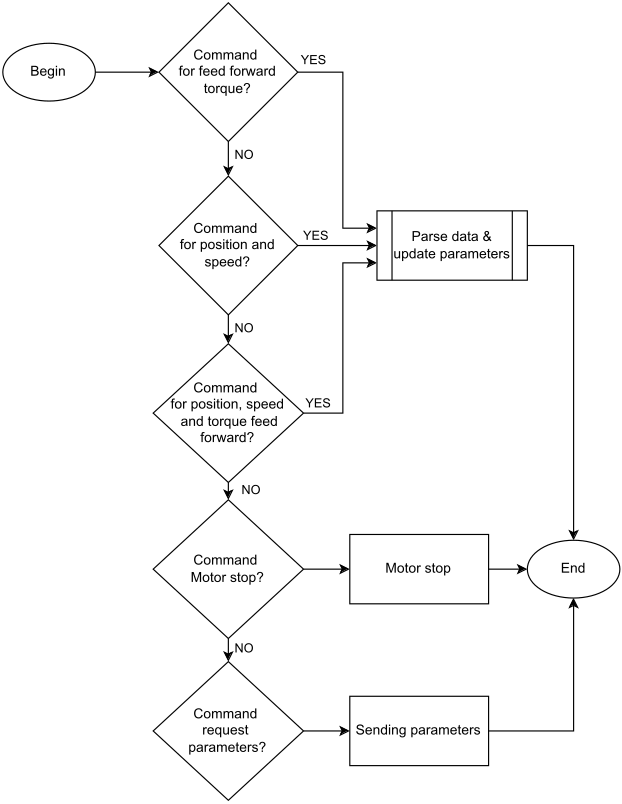
\includegraphics[width=0.8\textwidth]{Src/images/Receive parameters.png}
	\caption{"Receive parameters" subroutine operation algorithm}
	\label{AlgRecive}
\end{figure}

If a message from the Tactical Control Device (TCD) has been received, the process of extracting data from the message, containing information about the required position, speed, and controller coefficients, is executed. These data are used to calculate the vector control parameters. In case of receiving a data request message, parameters are sent to the sending device.
